%
%===============>>  ГРУППА 9-2 МОДУЛЬ 6  <<=============
%
\setmodule{6}

%BEGIN_FOLD % ====>>_____ Занятие 1 _____<<====
\begin{class}[number=1]
	\begin{listofex}
		\item В таблице даны размеры (с точностью до мм) четырёх листов, имеющих форматы \( A0 \), \( A1 \), \( A3 \), \( A4 \).
		\begin{center}
			\footnotesize
			\begin{tabular}{|c|c|c|}
				\hline
				\rowcolor{gray}\textbf{Номер листа}&\textbf{Длина(мм)}&\textbf{Ширина мм}\\
				\hline
				\( 1 \)&\( 297 \)&\( 210 \)\\
				\hline
				\( 2 \)&\( 420 \)&\( 297 \)\\
				\hline
				\( 3 \)&\( 1189 \)&\( 841 \)\\
				\hline
				\( 4 \)&\( 841 \)&\( 594 \)\\
				\hline
			\end{tabular}
		\end{center}
		Установите соответствие между форматами и номерами листов. В ответ запишите последовательность четырёх цифр, соответствующих номерам листов, без пробелов, запятых и дополнительных символов.
		\begin{center}
			\footnotesize
			\begin{tabular}{|c|c|c|c|}
				\hline
				\textbf{\( A0 \)}&\textbf{\( A1 \)}&\textbf{\( A3 \)}&\textbf{\( A4 \)}\\
				\hline
				\(  \)&\(  \)&\(  \)&\(  \)\\
				\hline
			\end{tabular}
		\end{center}
		Общепринятые форматы листов бумаги обозначают буквой \( A \) и цифрой: \( A0 \), \( A1 \), \( A2 \) и так далее. Лист формата \( A0 \) имеет форму прямоугольника, площадь которого равна \( 1 \) кв. м. Если лист формата А0 разрезать пополам параллельно меньшей стороне, получается два равных листа формата \( A1 \). Если лист \( A1 \) разрезать так же пополам, получается два листа формата \( A2 \). И так далее.\\
		\begin{minipage}[c]{0.35\textwidth}
			\includegraphics[align=t, width=\linewidth]{\picpath/G91M6L1}
		\end{minipage}\\
		Отношение большей стороны к меньшей стороне листа каждого формата одно и то же, поэтому листы всех форматов подобны. Это сделано специально для того, чтобы пропорции текста и его расположение на листе сохранялись при уменьшении или увеличении шрифта при изменении формата листа.
		\item Сколько листов формата \( A3 \) получится из одного листа формата \( A2 \)?
		\item Найдите площадь листа формата \( A1 \). Ответ дайте в квадратных сантиметрах.
		\item Найдите отношение длины меньшей стороны листа формата \( A3 \) к большей. Ответ округлите до десятых.
		\item Бумагу формата \( A5 \) упаковали в пачки по \( 500 \) листов. Найдите массу пачки, если масса бумаги площади \( 1 \) кв. м равна \( 80 \) г. Ответ дайте в граммах.
		\item Диагональ \( BD \) параллелограмма \( ABCD \) образует с его сторонами углы, равные \( 65\degree \) и \( 50\degree \). Найдите меньший угол параллелограмма.
		\item На продолжении стороны \( AD \) параллелограмма \( ABCD \) за точкой \( D \) отмечена точка \( E \) так, что \( DC=DE \). Найдите больший угол параллелограмма \( ABCD \), если \( \angle DEC=53\degree \). Ответ дайте в градусах.
		\item В параллелограмм вписана окружность. Найдите периметр параллелограмма, если одна из его сторон равна \( 6 \).
		\item Биссектриса угла \( A \) параллелограмма \( ABCD \) пересекает сторону \( BC \) в точке \( K \). Найдите периметр параллелограмма, если \( BK=6 \), \( CK=10 \).
		\item Площадь параллелограмма равна \( 40 \), а две его стороны равны \( 5 \) и \( 10 \). Найдите его высоты. В ответе укажите большую высоту.
		\item Расстояние от точки пересечения диагоналей ромба до одной из его сторон равно \( 19 \), а одна из диагоналей ромба равна \( 76 \). Найдите углы ромба.
		\item Периметр прямоугольника равен 56, а диагональ равна 27. Найдите площадь этого прямоугольника.
		\item Одна из сторон параллелограмма равна \( 12 \), другая равна \( 5 \), а косинус одного из углов равен \( \dfrac{2\sqrt{2}}{3} \). Найдите площадь параллелограмма.
		\item В ромбе сторона равна \( 10 \), одна из диагоналей --- \( 10\sqrt{2+\sqrt{2}} \), а угол, лежащий напротив этой диагонали, равен \( 135\degree \). Найдите площадь ромба, деленную на \( \sqrt{2} \).
		\item Площадь параллелограмма \( ABCD \) равна \( 132 \). Точка \( E \) --- середина стороны \( AB \). Найдите площадь треугольника \( CBE \).
		\item Площадь ромба равна \( 54 \), а периметр равен \( 36 \). Найдите высоту ромба.
	\end{listofex}
\end{class}
%END_FOLD

%BEGIN_FOLD % ====>>_____ Занятие 2 _____<<====
\begin{class}[number=2]
	\begin{listofex}
		\item Установите соответствие между объёмами помещения и номерами печей, для которых данный объём является наименьшим для отопления помещений. Заполните таблицу, в бланк ответов перенесите последовательность трёх цифр без пробелов, запятых и других дополнительных символов.
		\begin{center}
			\footnotesize
			\begin{tabular}{|c|c|c|c|}
				\hline
				Объём&\( 8 \)&\( 9 \)&\( 10 \)\\
				\hline
				Номер печи&\(  \)&\(  \)&\(  \)\\
				\hline
			\end{tabular}
		\end{center}
		Хозяин дачного участка строит баню с парным отделением. Парное отделение имеет размеры: длина \( 3,5 \) м, ширина \( 2,2 \) м, высота \( 2 \) м. Окон в парном отделении нет, для доступа внутрь планируется дверь шириной \( 60 \) см, высота дверного проёма \( 1,8 \) м. Для прогрева парного отделения можно использовать электрическую или дровяную печь. В таблице представлены характеристики трёх печей.
		\begin{center}
			\footnotesize
			\begin{tabular}{|c|c|c|c|c|}
				\hline
				\rowcolor{gray}\textbf{Номера печи}&\textbf{Тип}&\textbf{Объём помещения}&\textbf{Масса}&\textbf{Стоимость}\\
				\hline
				1&Дровяная&\( 8-12 \)&\( 40 \)&\( 18 000 \)\\
				\hline
				2&Дровяная&\( 10-16 \)&\( 48 \)&\( 19 500 \)\\
				\hline
				3&Электрическая&\( 9-15,5 \)&\( 15 \)&\( 15 000 \)\\
				\hline
			\end{tabular}
		\end{center}
		Для установки дровяной печи дополнительных затрат не потребуется. Установка электрической печи потребует подведения специального кабеля, что обойдётся в \( 6500 \) руб.
		\item Найдите объём парного отделения строящейся бани. Ответ дайте в кубических метрах.
		\item На сколько рублей покупка дровяной печи, подходящей по объёму парного отделения, обойдётся дороже электрической без учёта установки?
		\item Во сколько рублей обойдётся покупка электрической печи с установкой и доставкой, если доставка печи до дачного участка будет стоить \( 800 \) рублей?
		\item На дровяную печь, масса которой \( 48 \) кг, сделали скидку \( 10\% \). Сколько рублей стала стоить печь?
		\item Хозяин выбрал дровяную печь (рис. \( 1 \)). Чертёж передней панели печи показан на рисунке \( 2 \).
		\begin{center}
			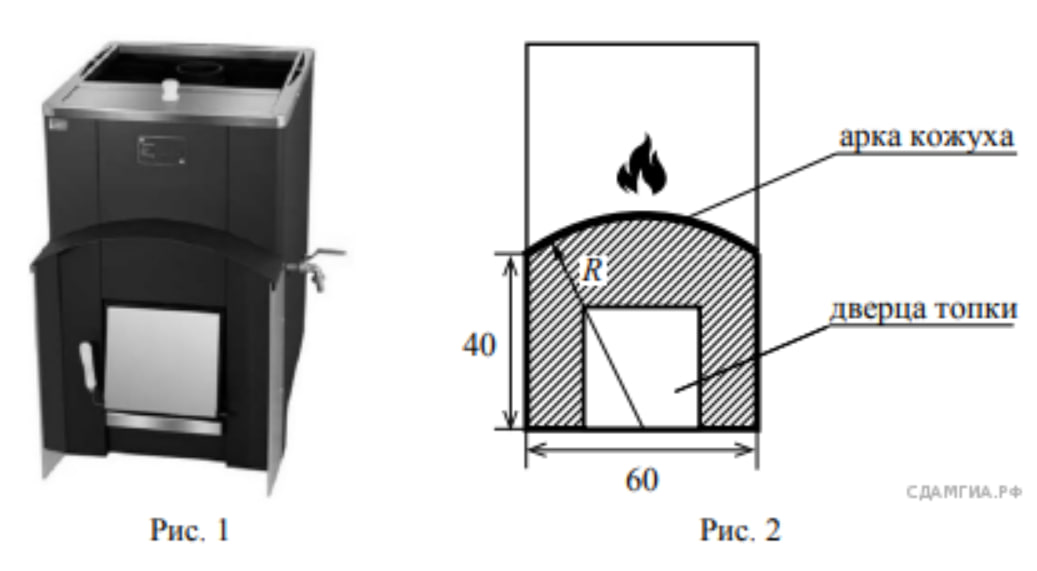
\includegraphics[align=t, width=0.5\linewidth]{\picpath/G91M6L2}
		\end{center}
		Печь снабжена кожухом вокруг дверцы топки. Верхняя часть кожуха выполнена в виде арки, приваренной к передней стенке печки по дуге окружности с центром в середине нижней части кожуха (см. рис. \( 2 \)). Для установки печки хозяину понадобилось узнать радиус закругления арки \( R \). Размеры кожуха в сантиметрах показаны на рисунке. Найдите радиус закругления арки в сантиметрах.
		\item Расстояние между пристанями \( A \) и \( B \) равно \( 80 \) км. Из \( A \) в \( B \) по течению реки отправился плот, а через \( 2 \) часа вслед за ним отправилась яхта, которая, прибыв в пункт \( B \), тотчас повернула обратно и возвратилась в \( A \). К этому времени плот прошел \( 22 \) км. Найдите скорость яхты в неподвижной воде, если скорость течения реки равна \( 2 \) км/ч. Ответ дайте в км/ч.
		\item Расстояние между городами \( A \) и \( B \) равно \( 750  \) км. Из города \( A \) в город \( B \) со скоростью \( 50 \) км/ч выехал первый автомобиль, а через три часа после этого навстречу ему из города \( B \) выехал со скоростью \( 70 \) км/ч второй автомобиль. На каком расстоянии от города \( A \) автомобили встретятся?	
		\item 
		\begin{minipage}[t]{\bodywidth}
			В параллелограмме \( ABCD \) проведены перпендикуляры \( DE \) и \( DF \) к диагонали \( AC \) (см. рис.). Докажите, что \( BFDE \) --- параллелограмм.
		\end{minipage}
		\hspace{0.02\linewidth}
		\begin{minipage}[t]{\picwidth}
			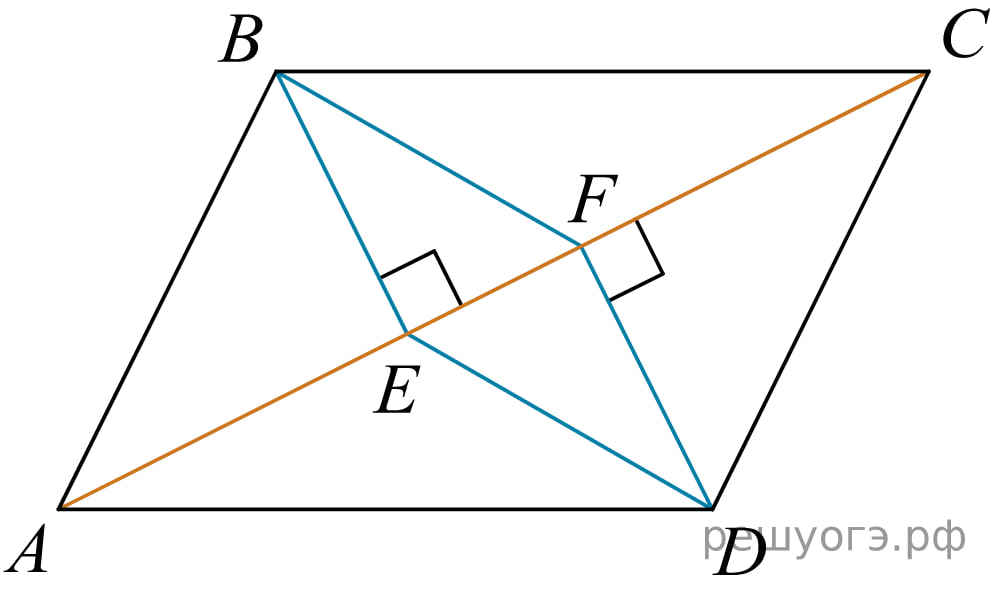
\includegraphics[align=t, width=\linewidth]{\picpath/G92M6L2}
		\end{minipage}
		\item Сторона \( BC \) параллелограмма \( ABCD \) вдвое больше стороны \( CD \). Точка \( L \) --- середина стороны \( BC \). Докажите, что \( DL \) --- биссектриса угла \( CDA \).
		\item В треугольнике \( ABC \) углы \( A \) и \( C \) равны \( 20\degree \) и \( 60\degree \) соответственно. Найдите угол между высотой \( BH \) и биссектрисой \( BD \). (Номер \( 23 \) из пробника, вариант \( 1 \))
		\item Окружность с центром на стороне \( AC \) треугольника \( ABC \) проходит через вершину \( C \) и касается прямой \( AB \) в точке \( B \). Найдите \( AC \), если диаметр окружности равен \( 7,5 \), а \( AB=2 \). (Номер \( 23 \) из пробника, вариант \( 2 \))
	\end{listofex}
\end{class}
%END_FOLD

%BEGIN_FOLD % ====>>_ Домашняя работа 1 _<<====
\begin{homework}[number=1]
	\begin{listofex}
		\item Найдите объём парного отделения строящейся бани (в куб. м).
		Хозяин дачного участка строит баню с парным отделением. Парное отделение имеет размеры: длина \( 3,9  \) м, ширина \( 2,1 \) м, высота \( 2 \) м. Для разогрева парного помещения можно использовать электрическую или дровяную печь. Три возможных варианта даны в таблице.
		\begin{center}
			\footnotesize
			\begin{tabular}{|c|c|c|c|c|}
				\hline
				\rowcolor{gray}\textbf{Номера печи}&\textbf{Тип}&\textbf{Объём помещения}&\textbf{Масса}&\textbf{Стоимость}\\
				\hline
				1&Дровяная&\( 9-14 \)&\( 42 \)&\( 19 100 \)\\
				\hline
				2&Дровяная&\( 12-18 \)&\( 49 \)&\( 20 500 \)\\
				\hline
				3&Электрическая&\( 10-17 \)&\( 16 \)&\( 16 000 \)\\
				\hline
			\end{tabular}
		\end{center}
		Для установки дровяной печи дополнительных затрат не потребуется. Установка электрической печи потребует подведения специального кабеля, что обойдётся в \( 6200 \) руб. Кроме того, хозяин подсчитал, что за год электрическая печь израсходует \( 2300 \) киловатт-часов электроэнергии по \( 3,5 \) руб. за \( 1 \) киловатт-час, а дровяная печь за год израсходует \( 1,6 \) куб. м дров, которые обойдутся по \( 1700 \) руб. за \( 1 \) куб. м.
		\item На сколько рублей дровяная печь, подходящая по отапливаемому объёму парного отделения, обойдётся дешевле электрической с учётом установки?
		\item На сколько рублей эксплуатация дровяной печи обойдётся дешевле эксплуатации электрической в течение года?
		\item Доставка печи из магазина до участка стоит \( 700 \) рублей. При покупке печи ценой выше \( 19 000 \) рублей магазин предлагает скидку \( 5\% \) на товар и \( 20\% \) на доставку. Сколько будет стоить покупка печи номер \( 2 \) вместе с доставкой на этих условиях?
		\item Хозяин выбрал дровяную печь. Чертёж печи показан ниже.
		\begin{minipage}[c]{0.2\textwidth}
			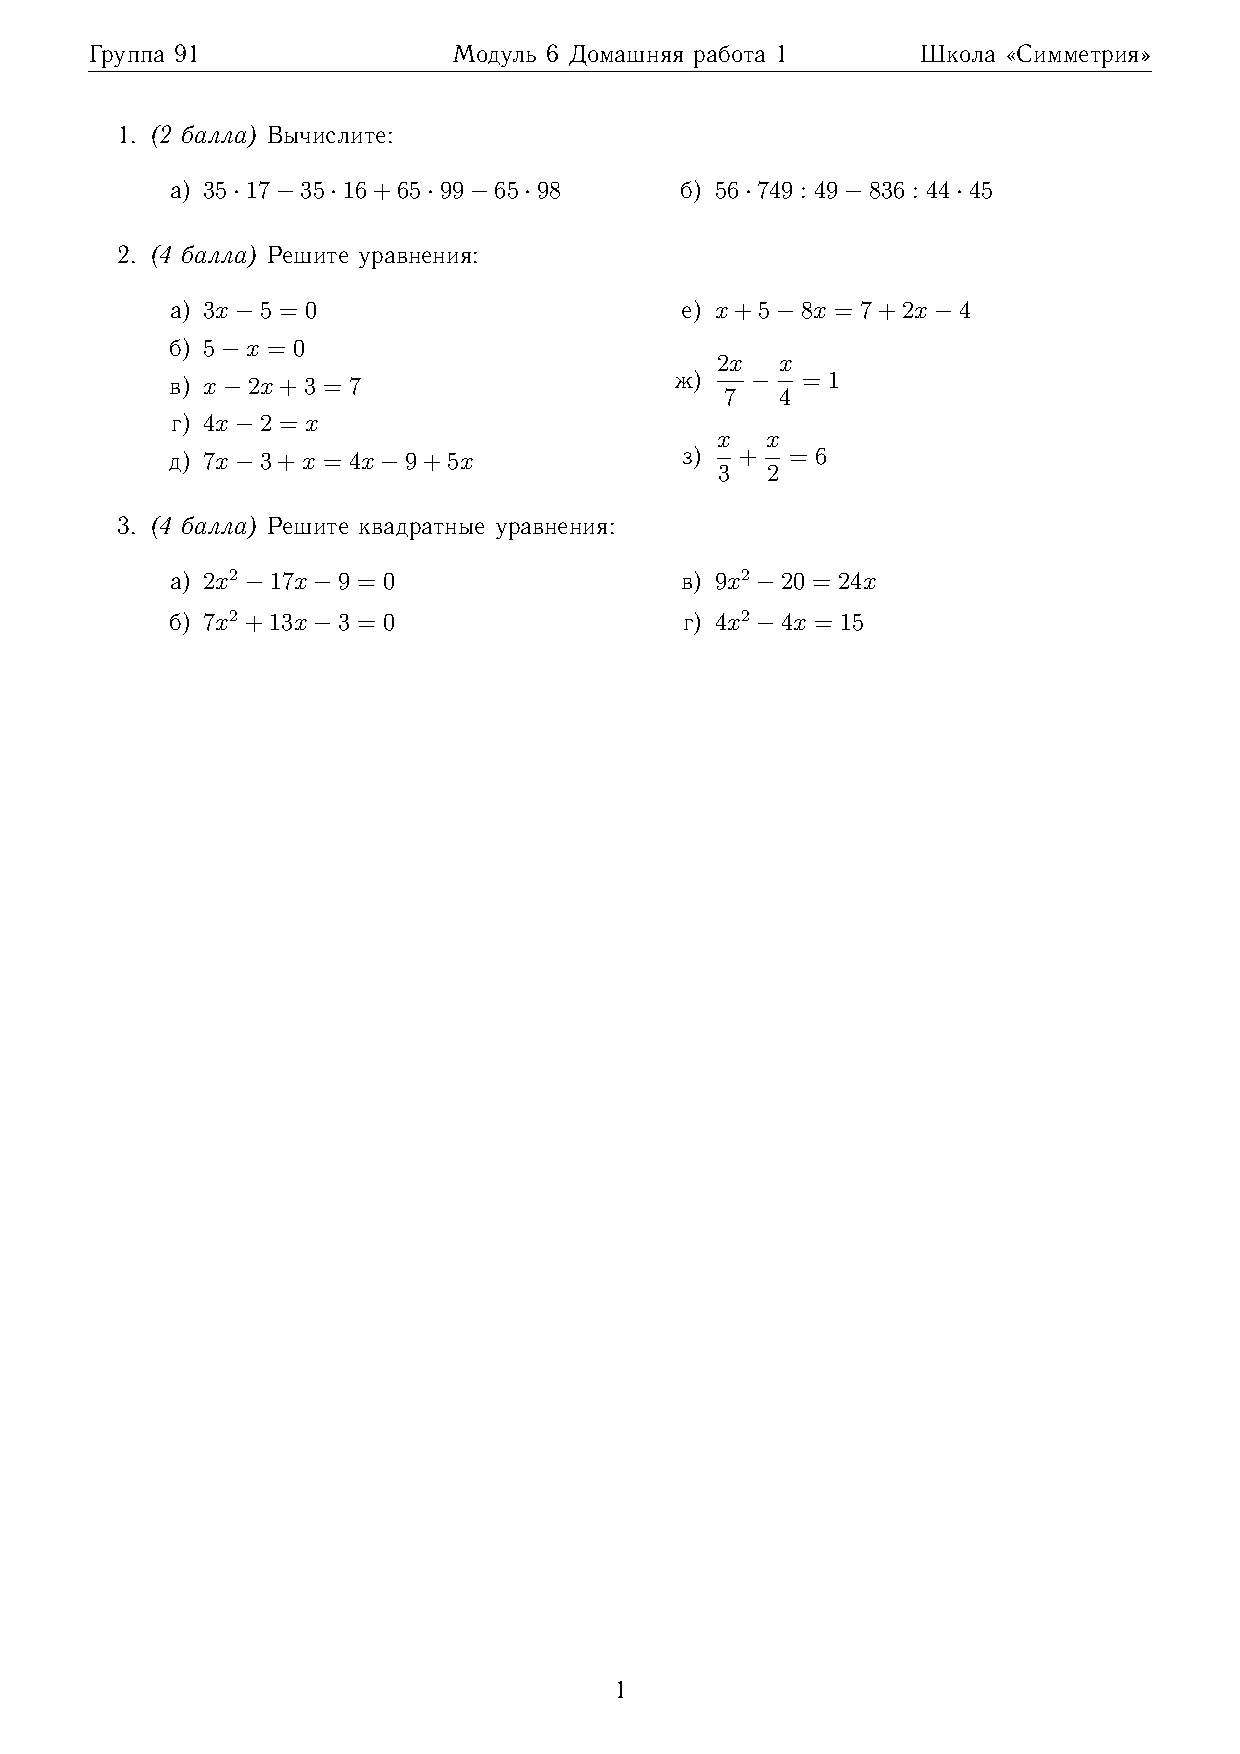
\includegraphics[align=t, width=\linewidth]{\picpath/G91M6H1}
		\end{minipage}\\
		Печь снабжена кожухом вокруг дверцы топки. Верхняя часть кожуха выполнена в виде арки, приваренной к передней стенке по дуге окружности. Для установки печки хозяину понадобилось узнать радиус закругления арки \( R \). Размеры кожуха в сантиметрах показаны на рисунке. Найдите радиус в сантиметрах.
		\item Пристани \( A \) и \( B \) расположены на реке, скорость течения которой на этом участке равна \( 3 \) км/ч. Лодка проходит туда и обратно без остановок со средней скоростью \( 8 \) км/ч. Найдите собственную скорость лодки.
		\item Площадь параллелограмма \( ABCD \) равна \( 132 \). Точка \( E \) --- середина стороны \( AB \). Найдите площадь треугольника \( CBE \).
		\item Площадь ромба равна \( 54 \), а периметр равен \( 36 \). Найдите высоту ромба.
		\item Биссектриса угла \( A \) параллелограмма \( ABCD \) пересекает его сторону \( BC \) в точке \( E \). Найдите площадь параллелограмма \( ABCD \), если \( BE=7 \), \( EC=3 \), а \( \angle ABC =150\degree \).
		\item Найдите значение выражения:
		\begin{tasks}(2)
			\task \( \sqrt{7\cdot3^4}\cdot\sqrt{7\cdot2^2} \)
			\task \( \sqrt{3^2\cdot5^4\cdot11^2} \)
			\task \( \sqrt{40\cdot60\cdot75} \)
			\task \( (4\sqrt{3})^2 \)
		\end{tasks}
	\end{listofex}
\end{homework}
%END_FOLD

%BEGIN_FOLD % ====>>_____ Занятие 3 _____<<====
\begin{class}[number=3]
	\begin{listofex}
		\item Завод допускает установку шин с другими маркировками. В таблице показаны разрешённые размеры шин.
		\begin{center}
			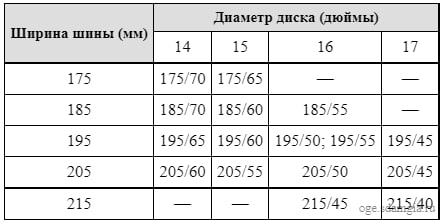
\includegraphics[align=t, width=0.5\linewidth]{\picpath/G91M6L3-1}
		\end{center}
		Шины какой наименьшей ширины можно устанавливать на автомобиль, если диаметр диска равен \( 16 \) дюймам? Ответ дайте в миллиметрах.
		\begin{center}
			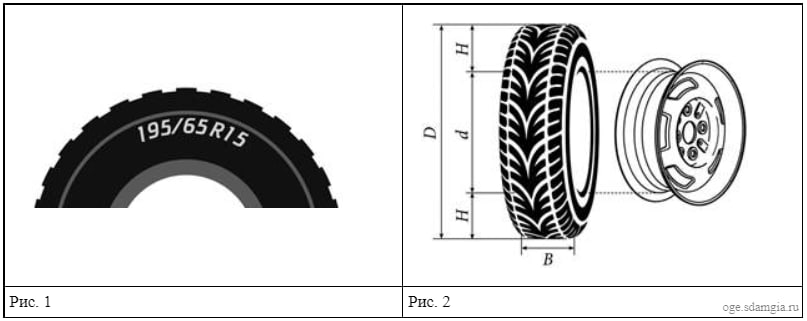
\includegraphics[align=t, width=0.5\linewidth]{\picpath/G91M6L3-2}
		\end{center}
		Автомобильное колесо, как правило, представляет из себя металлический диск с установленной на него резиновой шиной. Диаметр диска совпадает с диаметром внутреннего отверстия в шине.\\
		Для маркировки автомобильных шин применяется единая система обозначений. Например, \( 195/65 R15 \) (рис. \( 1 \)). Первое число (число \( 195 \) в приведённом примере) обозначает ширину шины в миллиметрах (параметр \( B \) на рисунке \( 2 \)). Второе число (число \( 65 \) в приведённом примере)  — процентное отношение высоты боковины (параметр на рисунке \( 2 \)) к ширине шины, то есть \( 100\cdot\dfrac{H}{B} \). \\
		Последующая буква обозначает тип конструкции шины. В данном примере буква \( R \) означает, что шина радиальная, то есть нити каркаса в боковине шины расположены вдоль радиусов колеса. На всех легковых автомобилях применяются шины радиальной конструкции.\\		
		За обозначением типа конструкции шины идёт число, указывающее диаметр диска колеса \( d \) в дюймах (в одном дюйме \( 25,4 \) мм). Таким образом, общий диаметр колеса \( D \) легко найти, зная диаметр диска и высоту боковины.\\		
		Возможны дополнительные маркировки, обозначающие допустимую нагрузку на шину, сезонность использования, тип дорожного покрытия и другие параметры.		
		Завод производит легковые автомобили определённой модели и устанавливает на них колёса с шинами маркировки \( 185/60 R15 \).
		\item На сколько миллиметров радиус колеса с шиной маркировки \( 220/60 R16 \) меньше, чем радиус колеса с шиной маркировки \( 245/55 R16 \)?
		\item Найдите диаметр колеса автомобиля, выходящего с завода. Ответ дайте в миллиметрах.
		\item На сколько процентов увеличится пробег автомобиля при одном обороте колеса, если заменить колёса, установленные на заводе, колёсами с шинами маркировки \( 175/60 R14 \)? Результат округлите до десятых.
		\item Найдите угол \( ADC \) равнобедренной трапеции \( ABCD \), если диагональ \( AC \) образует с основанием \( BC \) и боковой стороной \( AB \) углы, равные \( 30\degree \) и \( 50\degree \) соответственно.
		\item Сумма двух углов равнобедренной трапеции равна \( 140\degree \). Найдите больший угол трапеции. Ответ дайте в градусах.
		\item Найдите меньший угол равнобедренной трапеции, если два ее угла относятся как \( 1:2 \). Ответ дайте в градусах.
		\item Основания трапеции равны \( 4 \) см и \( 10 \) см. Диагональ трапеции делит среднюю линию на два отрезка. Найдите длину большего из них.
		\item Средняя линия трапеции равна \( 11 \), а меньшее основание равно \( 5 \). Найдите большее основание трапеции.
		\item Тангенс острого угла прямоугольной трапеции равен \( \dfrac{5}{6} \).  Найдите её большее основание, если меньшее основание равно высоте и равно \( 15 \).
		\item Найдите угол \( ABC \) равнобедренной трапеции \( ABCD \), если диагональ \( AC \) образует с основанием \( AD \) и боковой стороной \( CD \) углы, равные \( 20\degree \) и \( 100\degree \) соответственно.
		\item Основания трапеции равны \( 4 \) и \( 10 \), а высота равна \( 5 \). Найдите площадь этой трапеции.
		\item Один из углов прямоугольной трапеции равен \( 64\degree \). Найдите больший угол этой трапеции. Ответ дайте в градусах.
		\item Диагонали \( AC \) и \( BD \) трапеции \( ABCD \) с основаниями \( BC \) и \( AD \) пересекаются в точке \( O \), \( DC=3 \), \( AD=7 \), \( AC=20 \). Найдите \( AO \).
		\item Постройте график функции \( y=x^2-|4x+3| \) и определите, при каких значениях \( m \) прямая \( y=m \) имеет с графиком ровно три общие точки.
	\end{listofex}
\end{class}
%END_FOLD

%BEGIN_FOLD % ====>>_____ Занятие 4 _____<<====
\begin{class}[number=4]
	\begin{listofex}
		\item Какое наименьшее количество дуг нужно заказать, чтобы расстояние между соседними дугами было не более \( 60 \) см?
		\begin{center}
			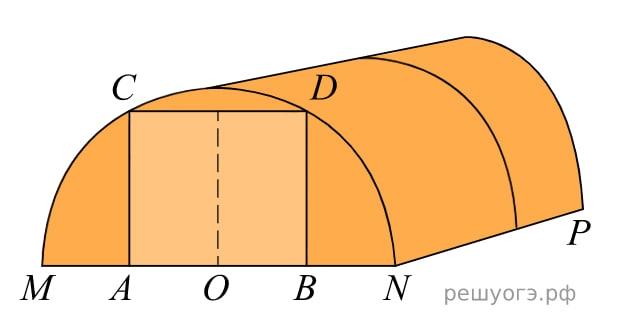
\includegraphics[align=t, width=0.5\linewidth]{\picpath/G92M6L4}
		\end{center}
		Алексей Юрьевич решил построить на дачном участке теплицу длиной \( NP=4,5 \) м. Для этого он сделал прямоугольный фундамент. Для каркаса теплицы Алексей Юрьевич заказывает металлические дуги в форме полуокружностей длиной \( 5,2 \) м каждая и плёнку для обтяжки. В передней стенке планируется вход, показанный на рисунке прямоугольником \( ACDB \). Точки \( A \) и \( B \) --- середины отрезков \( MO \) и \( ON \) соответственно.
		\item Найдите примерную ширину \( MN \) теплицы в метрах. Число \( \pi  \) возьмите равным \( 3,14 \). Результат округлите до десятых.
		\item Найдите примерную площадь участка внутри теплицы в квадратных метрах. Ответ округлите до целых.
		\item Сколько квадратных метров плёнки нужно купить для теплицы с учётом передней и задней стенок, включая дверь? Для крепежа плёнку нужно покупать с запасом \( 10\% \). Число \( \pi \) возьмите равным \( 3,14 \). Ответ округлите до целых.
		\item Найдите примерную высоту входа в теплицу в метрах. Число \( \pi \) возьмите равным \( 3,14 \). Ответ округлите до десятых.
		\item Основания равнобедренной трапеции равны \( 8 \) и \( 18 \), а периметр равен \( 56 \). Найдите площадь трапеции.
		\item Прямая, параллельная основаниям \( MP \) и \( NK \) трапеции \( MNKP \), проходит через точку пересечения диагоналей трапеции и пересекает её боковые стороны \( MN \) и \( KP \) в точках  \( A \) и \( B \) соответственно. Найдите длину отрезка \( AB \), если \( MP=40 \) см, \( NK=24 \) см.
		\item В трапеции \( ABCD \) основание \( AD \) вдвое больше основания \( BC \) и вдвое больше боковой стороны \( CD \). Угол \( ADC \) равен \( 60\degree \), сторона \( AB \) равна \( 2 \). Найдите площадь трапеции.
		\item Каждое основание \( AD \) и \( DC \) трапеции \( ABCD \) продолжено в обе стороны. Биссектрисы внешних углов \( A \) и \( B \) этой трапеции пересекаются в точке \( K \), биссектрисы внешних углов \( C \) и \( D \) пересекаются в точке \( E \). Найдите периметр трапеции \( ABCD \), если длина отрезка \( KE \) равна \( 28 \).
		\item В трапеции \( ABCD \) основание \( AD \) вдвое больше основания \( BC \) и вдвое больше боковой стороны \( CD \). Угол \( ADC \) равен \( 60\degree \), сторона \( AB \) равна \( 1 \). Найдите площадь трапеции.
		\item Прямая, параллельная основаниям \( AD \) и \( BC \) трапеции \( ABCD \), проходит через точку пересечения диагоналей трапеции и пересекает ее боковые стороны \( AB \) и \( CD \) в точках \( E \) и \( F \) соответственно. Найдите длину отрезка \( EF \), если \( AD=10 \) см, \( BC=15 \) см.
	\end{listofex}
\end{class}
%END_FOLD

%BEGIN_FOLD % ====>>_ Домашняя работа 2 _<<====
\begin{homework}[number=2]
	\begin{listofex}
		\item В таблице даны размеры (с точностью до мм) четырёх листов, имеющих форматы \( A0 \), \( A1 \), \( A3 \), \( A4 \).
		\begin{center}
			\footnotesize
			\begin{tabular}{|c|c|c|}
				\hline
				\rowcolor{gray}\textbf{Номер листа}&\textbf{Длина(мм)}&\textbf{Ширина мм}\\
				\hline
				\( 1 \)&\( 297 \)&\( 210 \)\\
				\hline
				\( 2 \)&\( 420 \)&\( 297 \)\\
				\hline
				\( 3 \)&\( 1189 \)&\( 841 \)\\
				\hline
				\( 4 \)&\( 841 \)&\( 594 \)\\
				\hline
			\end{tabular}
		\end{center}
		Установите соответствие между форматами и номерами листов. В ответ запишите последовательность четырёх цифр, соответствующих номерам листов, без пробелов, запятых и дополнительных символов.
		\begin{center}
			\footnotesize
			\begin{tabular}{|c|c|c|c|}
				\hline
				\textbf{\( A0 \)}&\textbf{\( A1 \)}&\textbf{\( A3 \)}&\textbf{\( A4 \)}\\
				\hline
				\(  \)&\(  \)&\(  \)&\(  \)\\
				\hline
			\end{tabular}
		\end{center}
		Общепринятые форматы листов бумаги обозначают буквой \( A \) и цифрой: \( A0 \), \( A1 \), \( A2 \) и так далее. Лист формата \( A0 \) имеет форму прямоугольника, площадь которого равна \( 1 \) кв. м. Если лист формата А0 разрезать пополам параллельно меньшей стороне, получается два равных листа формата \( A1 \). Если лист \( A1 \) разрезать так же пополам, получается два листа формата \( A2 \). И так далее.
		\begin{center}
			\includegraphics[align=t, width=0.4\linewidth]{../pics/G91M6L1}
		\end{center}
		Отношение большей стороны к меньшей стороне листа каждого формата одно и то же, поэтому листы всех форматов подобны. Это сделано специально для того, чтобы пропорции текста и его расположение на листе сохранялись при уменьшении или увеличении шрифта при изменении формата листа.
		\item Сколько листов формата \( A5 \) получится из одного листа формата \( A1 \)?
		\item Найдите площадь листа формата \( A6 \). Ответ дайте в квадратных сантиметрах.
		\item Найдите отношение длины большей стороны листа формата \( A2 \) к меньшей. Ответ округлите до десятых.
		\item Бумагу формата \( A3 \) упаковали в пачки по \( 250 \) листов. Найдите массу пачки, если масса бумаги площади \( 1 \) кв. м равна \( 120 \) г. Ответ дайте в граммах.
		\item Диагональ трапеции делит её среднюю линию на отрезки, равные \( 4 \) см и \( 3 \) см. Найдите меньшее основание трапеции.
		\item Найдите больший угол равнобедренной трапеции \( ABCD \), если диагональ \( AC \) образует с основанием \( AD \) и боковой стороной \( AB \) углы, равные \( 33\degree \) и \( 13\degree  \) соответственно. Ответ дайте в градусах.
		\item Основания трапеции равны \( 3 \) и \( 9 \), а высота равна \( 5 \). Найдите среднюю линию этой трапеции.
		\item Найдите меньший угол равнобедренной трапеции \( ABCD \), если диагональ \( AC \) образует с основанием \( BC \) и боковой стороной \( CD \) углы, равные \( 30\degree \) и \( 105\degree \) соответственно.
		\item Решите уравнение:
		\[(x-2)(x-3)(x-5)=(x-2)(x-4)(x-5)\]
		\item Прямая, параллельная основаниям \( MP \) и \( NK \) трапеции \( MNKP \), проходит через точку пересечения диагоналей трапеции и пересекает её боковые стороны \( MN \) и \( KP \) в точках \( A \) и \( B \) соответственно. Найдите длину отрезка \( AB \), если \( MP=24 \) см, \( NK=16 \) см.
	\end{listofex}
\end{homework}
%END_FOLD

%BEGIN_FOLD % ====>>_____ Занятие 5 _____<<====
\begin{class}[number=5]
	\begin{listofex}
		\item Центральный угол \( AOB \) опирается на хорду \( AB \) длиной \( 6 \). При этом угол \( OAB \) равен \( 60\degree \). Найдите радиус окружности.
		\item В окружности с центром в точке \( O \) проведены диаметры \( AD \) и \( BC \), угол \( OCD \) равен \( 30\degree \). Найдите величину угла \( OAB \).
		\item Найдите градусную меру тупого центрального угла \( MON \), если известно, \( NP \) --- диаметр, а градусная мера угла \( MNP \) равна \( 18\degree \).
		\item Найдите вписанный угол \( DEF \), если градусные меры дуг \( DE \) и \( EF \) равны \( 150\degree \) и \( 68\degree \) соответственно.
		\item Найдите градусную меру угла \( ACB \), если известно, что \( BC \) является диаметром окружности, а градусная мера центрального угла \( AOC \) равна \( 96\degree \).
		\item В окружности с центром \( O \) \( AC \) и \( BD \) --- диаметры. Угол \( ACB \) равен \( 26\degree \). Найдите угол \( AOD \). Ответ дайте в градусах.
		\item Прямоугольный треугольник с катетами \( 5 \) см и \( 12 \) см вписан в окружность. Чему равен радиус этой окружности?
		\item Точки \( A \) и \( B \) делят окружность на две дуги, длины которых относятся как \( 9:11 \). Найдите величину центрального угла, опирающегося на меньшую из дуг. Ответ дайте в градусах.
		\item Величина центрального угла \( AOD \) равна \( 110\degree \). Найдите величину вписанного угла \( ACB \). Ответ дайте в градусах.
		\item Точки \( A \), \( B \), \( C \) и \( D \) лежат на одной окружности так, что хорды \( AB \) и \( CD \) взаимно перпендикулярны, а угол \( BDC=25\degree \) . Найдите величину угла \( ACD \).
		\item В треугольнике \( ABC \) угол \( B \) равен \( 72\degree \), угол \( C \) равен \( 63\degree \), \( BC=2\sqrt{2} \). Найдите радиус описанной около этого треугольника окружности.
		\item Окружность с центром на стороне \( AC \) треугольника \( ABC \) проходит через вершину \( C \) и касается прямой \( AB \) в точке \( B \). Найдите \( AC \), если диаметр окружности равен \( 7,5 \), а \( AB=2 \).
		\item В окружности с центром \( O \) проведены две хорды \( AB \) и \( CD \) так, что центральные углы \( AOB \) и \( COD \) равны. На эти хорды опущены перпендикуляры \( OK \) и \( OL \). Докажите, что \( OK \) и \( OL \) равны.
		\item Окружности с центрами в точках \( I \) и \( J \) пересекаются в точках \( A \) и \( B \), причём точки \( I \) и \( J \) лежат по одну сторону от прямой \( AB \). Докажите, что отрезки \( AB \) и \( IJ \) перпендикулярны.
		\item В окружности с центром \( O \) проведены две равные хорды \( KL \) и \( MN \). На эти хорды опущены перпендикуляры \( OH \) и \( OS \). Докажите, что \( OH \) и \( OS \) равны.
		\item На изготовление \( 231 \) детали ученик тратит на \( 11 \) часов больше, чем мастер на изготовление \( 462 \) таких же деталей. Известно, что ученик за час делает на \( 4 \) детали меньше, чем мастер. Сколько деталей в час делает ученик?
		\item Две трубы наполняют бассейн за \( 6 \) часов \( 18 \) минут, а одна первая труба наполняет бассейн за \( 9 \) часов. За сколько часов наполняет бассейн одна вторая труба?
	\end{listofex}
\end{class}
%END_FOLD

%BEGIN_FOLD % ====>>_____ Занятие 6 _____<<====
\begin{class}[number=6]
	\begin{listofex}
		\item Радиус окружности, вписанной в трапецию, равен \( 16 \). Найдите высоту этой трапеции.
		\item К окружности с центром в точке \( O \) проведены касательная \( AB \) и секущая \( AO \). Найдите радиус окружности, если \( AB=12 \) см, \( AO=13 \) см.
		\item Прямая касается окружности в точке \( K \). Точка \( O \) --- центр окружности. Хорда \( KM \) образует с касательной угол, равный \( 83\degree \). Найдите величину угла \( OMK \). Ответ дайте в градусах.
		\item На окружности отмечены точки \( A \) и \( B \) так, что меньшая дуга \( AB \) равна \( 72\degree \). Прямая \( BC \) касается окружности в точке \( B \) так, что угол \( ABC \) острый. Найдите угол \( ABC \). Ответ дайте в градусах.
		\item На отрезке \( AB \) выбрана точка \( C \) так, что \( AC=75 \) и \( BC=10 \). Построена окружность с центром \( A \), проходящая через \( C \) Найдите длину отрезка касательной, проведённой из точки \( B \) к этой окружности.		
		\item Через точку \( A \), лежащую вне окружности, проведены две прямые. Одна прямая касается окружности в точке \( K \). Другая прямая пересекает окружность в точках \( B \) и \( C \), причём \( AB=2 \), \( AC=8 \). Найдите \( AK \).
		\item Хорды \( AC \) и \( BD \) окружности пересекаются в точке \( P \), \( BP=15 \), \( CP=6 \), \( DP=10 \). Найдите \( AP \).
		\item Радиус вписанной в квадрат окружности равен \( 2\sqrt{2} \) . Найдите диагональ этого квадрата.
		\item Отрезок \( AB=40 \) касается окружности радиуса \( 75 \) с центром \( O \) в точке \( B \). Окружность пересекает отрезок \( AO \) в точке \( D \). Найдите \( AD \).
		\item Радиус окружности, описанной около равностороннего треугольника, равен \( 6 \). Найдите высоту этого треугольника.
		\item Длина хорды окружности равна \( 72 \), а расстояние от центра окружности до этой хорды равно \( 27 \). Найдите диаметр окружности.
		\item Из точки \( A \) проведены две касательные к окружности с центром в точке \( O \). Найдите радиус окружности, если угол между касательными равен \( 60\degree \), а расстояние от точки \( A \) до точки \( O \) равно \( 8 \).
		\item Радиус окружности, вписанной в равносторонний треугольник, равен \( 5 \). Найдите высоту этого треугольника.
		\item Касательные в точках \( A \) и \( B \) к окружности с центром \( O \) пересекаются под углом \( 72\degree \). Найдите угол \( ABO \). Ответ дайте в градусах.
		\item Отрезки \( AB \) и \( CD \) являются хордами окружности. Найдите расстояние от центра окружности до хорды \( CD \), если \( AB=18 \), \( CD=24 \), а расстояние от центра окружности до хорды \( AB \) равно \( 12 \).
		\item Радиус окружности, описанной около квадрата, равен \( 44\sqrt{2} \). Найдите радиус окружности, вписанной в этот квадрат.
		\item Радиус окружности, вписанной в равносторонний треугольник, равен \( 2\sqrt{3} \). Найдите длину стороны этого треугольника.
		\item Вершины треугольника делят описанную около него окружность на три дуги, длины которых относятся как \( 3:4:11 \). Найдите радиус окружности, если меньшая из сторон равна \( 14 \).
		\item В окружность вписан равносторонний восьмиугольник \( ABCDEFGH \). Найдите величину угла \( ACE \).
		\item Боковая сторона равнобедренного треугольника равна \( 4 \). Угол при вершине, противолежащий основанию, равен \( 120\degree \). Найдите диаметр окружности, описанной около этого треугольника.
		\item Три окружности с центрами \( O_1 \), \( O_2 \) и \( O_3 \) и радиусами \( 2,5 \), \( 0,5 \) и \( 4,5 \) соответственно попарно касаются внешним образом. Найдите угол \( O_1O_2O_3 \).
		\item Две окружности с центрами \( O_1 \) и \( O_3 \) и радиусами \( 4,5 \) и \( 2,5 \) касаются друг с другом внешним образом и внутренним образом касаются окружности с центром \( O_2 \) радиусом \( 7,5 \). Найдите угол \( O_1O_2O_3 \).
		\item Основание \( AC \) равнобедренного треугольника \( ABC \) равно \( 12 \). Окружность радиуса \( 8 \) с центром вне этого треугольника касается продолжений боковых сторон треугольника и касается основания \( AC \) в его середине. Найдите радиус окружности, вписанной в треугольник \( ABC \).
	\end{listofex}
\end{class}
%END_FOLD

%BEGIN_FOLD % ====>>_ Домашняя работа 3 _<<====
\begin{homework}[number=3]
	\begin{listofex}
		\item На сколько миллиметров будет отличаться диаметр колеса, если заменить колёса, установленные на заводе, колёсами с шинами маркировки \( 195/50 R15 \)?
		\begin{center}
			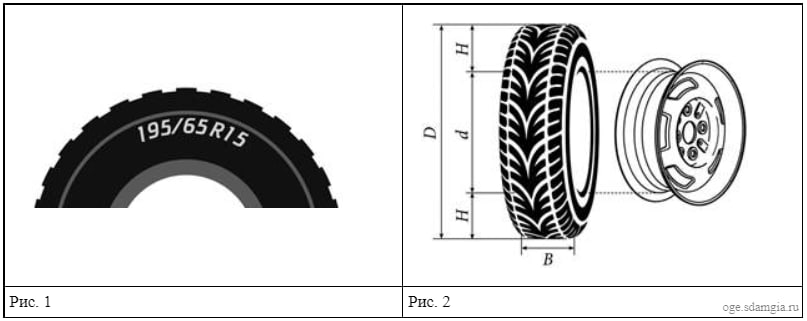
\includegraphics[align=t, width=0.5\linewidth]{\picpath/G91M6L3-2}
		\end{center}
		Автомобильное колесо, как правило, представляет из себя металлический диск с установленной на него резиновой шиной. Диаметр диска совпадает с диаметром внутреннего отверстия в шине.\\
		Для маркировки автомобильных шин применяется единая система обозначений. Например, \( 195/65 R15 \) (рис. \( 1 \)). Первое число (число \( 195 \) в приведённом примере) обозначает ширину шины в миллиметрах (параметр \( B \) на рисунке \( 2 \)). Второе число (число \( 65 \) в приведённом примере)  — процентное отношение высоты боковины (параметр на рисунке \( 2 \)) к ширине шины, то есть \( 100\cdot\dfrac{H}{B} \). \\
		Последующая буква обозначает тип конструкции шины. В данном примере буква \( R \) означает, что шина радиальная, то есть нити каркаса в боковине шины расположены вдоль радиусов колеса. На всех легковых автомобилях применяются шины радиальной конструкции.\\		
		За обозначением типа конструкции шины идёт число, указывающее диаметр диска колеса \( d \) в дюймах (в одном дюйме \( 25,4 \) мм). Таким образом, общий диаметр колеса \( D \) легко найти, зная диаметр диска и высоту боковины.\\		
		Возможны дополнительные маркировки, обозначающие допустимую нагрузку на шину, сезонность использования, тип дорожного покрытия и другие параметры.		
		Завод производит легковые автомобили определённой модели и устанавливает на них колёса с шинами маркировки \( 185/60 R15 \).
		\item На сколько процентов изменится пробег автомобиля при одном обороте колеса, если заменить колёса, установленные на заводе, колёсами с шинами маркировки \( 175/60 R14 \)? Результат округлите до десятых.
		\item Две трубы наполняют бассейн за \( 8 \) часов \( 45 \) минут, а одна первая труба наполняет бассейн за \( 21 \) час. За сколько часов наполняет бассейн одна вторая труба?
		\item К окружности с центром в точке \( O \) проведены касательная \( AB \) и секущая \( AO \). Найдите радиус окружности, если \( AB=51 \), \( AO=85 \).
		\item Сторона равностороннего треугольника равна \( 12\sqrt{3} \) . Найдите радиус окружности, вписанной в этот треугольник.
		\item Радиус окружности, описанной около квадрата, равен \( 24\sqrt{2} \) . Найдите радиус окружности, вписанной в этот квадрат.
		\item В окружности через середину \( O \) хорды \( AC \) проведена хорда \( BD \) так, что дуги \( AB \) и \( CD \) равны. Докажите, что \( O \) --- середина хорды \( BD \).
		\item Постройте график функции \( y=x^2-6|x|+2x \)  и определите, при каких значениях \( c \) прямая \( y=c \) имеет с графиком ровно три общие точки.
	\end{listofex}
\end{homework}
%END_FOLD

%BEGIN_FOLD % ====>>_____ Занятие 7 _____<<====
\begin{class}[number=7]
	\begin{listofex}
		\item Длина зонта в сложенном виде равна \( 25 \) см и складывается из длины ручки (рис. \( 3 \)) и трети длины спицы (зонт в три сложения). Найдите длину спицы, если длина ручки зонта равна \( 6,2 \) см.\\\\
		Два друга Петя и Вася задумались о том, как рассчитать площадь поверхности зонта.\\
		На первый взгляд зонт кажется круглым, а его купол напоминает часть сферы (сферический сегмент). Но если присмотреться, то видно, что купол зонта состоит из восьми отдельных клиньев, натянутых на каркас из восьми спиц (рис. \( 1 \)). Сферическая форма в раскрытом состоянии достигается за счёт гибкости спиц и эластичности ткани, из которой изготовлен зонт.
		Петя и Вася сумели измерить расстояние между концами соседних спиц \( a \). Оно оказалось равно \( 38 \) см. Высота купола зонта \( h \) (рис. \( 2 \)) оказалась равна \( 25 \) см, а расстояние \( d \) между концами спиц, образующих дугу окружности, проходящей через вершину зонта, --- ровно \( 100 \) см.
		\begin{center}
			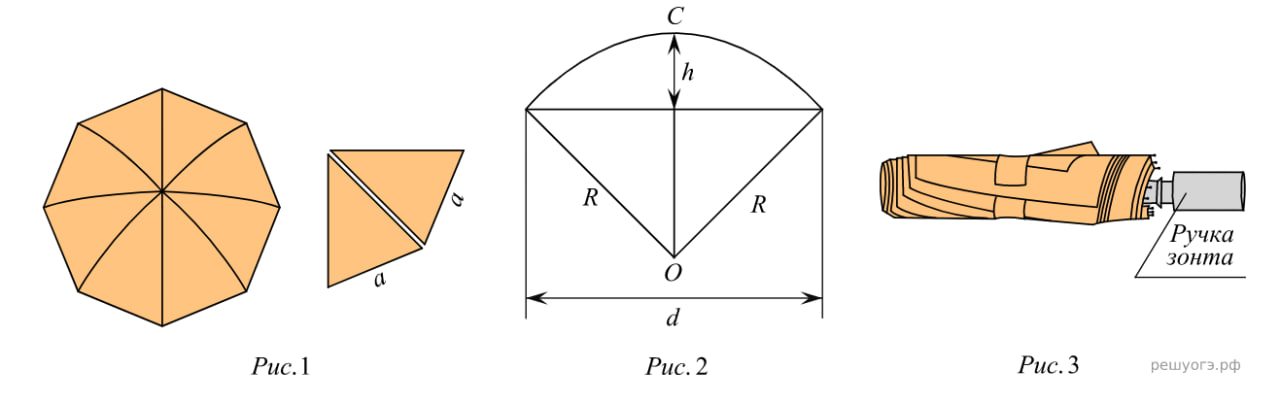
\includegraphics[align=t, width=0.5\linewidth]{\picpath/G91M6L7}
		\end{center}
		\item Поскольку зонт сшит из треугольников, рассуждал Петя, площадь его поверхности можно найти как сумму площадей треугольников. Вычислите площадь поверхности зонта методом Пети, если высота каждого равнобедренного треугольника, проведённая к основанию, равна \( 53,1 \) см. Ответ дайте в квадратных сантиметрах с округлением до десятков.
		\item Вася предположил, что купол зонта имеет форму сферического сегмента. Вычислите радиус \( R \) сферы купола, зная, что \( OC=R \) (рис. \( 2 \)). Ответ дайте в сантиметрах.
		\item Вася нашёл площадь купола зонта как площадь поверхности сферического сегмента по формуле \( S=2\pi Rh \),  где \( R \) --- радиус сферы, a \( h \) --- высота сегмента. Рассчитайте площадь поверхности купола способом Васи. Число \( \pi \) округлите до \( 3,14 \). Ответ дайте в квадратных сантиметрах с округлением до целого.
		\item Рулон ткани имеет длину \( 35 \) м и ширину \( 80 \) см. На фабрике из этого рулона были вырезаны треугольные клинья для \( 29 \) зонтов, таких же, как зонт, который был у Пети и Васи. Каждый треугольник с учётом припуска на швы имеет площадь \( 1050 \) кв. см. Оставшаяся ткань пошла в обрезки. Сколько процентов ткани рулона пошло в обрезки?
		\item Радиус круга равен \( 1 \). Найдите его площадь, деленную на \( \pi \).
		\item Найдите площадь кругового сектора, если радиус круга равен \( 3 \), а угол сектора равен \( 120\degree \). В ответе укажите площадь, деленную на \( \pi \).
		\item Найдите площадь кругового сектора, если длина ограничивающей его дуги равна \( 6\pi \), а угол сектора равен \( 120\degree \). В ответе укажите площадь, деленную на \( \pi \).
		\item Радиус круга равен \( 3 \), а длина ограничивающей его окружности равна \( 6\pi \). Найдите площадь круга. В ответ запишите площадь, деленную на \( \pi \).
		\item Найдите площадь кругового сектора, если длина ограничивающей его дуги равна \( 6\pi \), угол сектора равен \( 120\degree \), а радиус круга равен \( 9 \). В ответе укажите площадь, деленную на \( \pi \).
		\item Три окружности с центрами \( O_1 \), \( O_2 \) и \( O_3 \) и радиусами \( 2,5 \), \( 0,5 \) и \( 4,5 \) соответственно попарно касаются внешним образом. Найдите угол \( O_1O_2O_3 \).
		\item Две окружности с центрами \( O_1 \) и \( O_3 \) и радиусами \( 4,5 \) и \( 2,5 \) касаются друг с другом внешним образом и внутренним образом касаются окружности с центром \( O_2 \) радиусом \( 7,5 \). Найдите угол \( O_1O_2O_3 \).
		\item Основание \( AC \) равнобедренного треугольника \( ABC \) равно \( 12 \). Окружность радиуса \( 8 \) с центром вне этого треугольника касается продолжений боковых сторон треугольника и касается основания \( AC \) в его середине. Найдите радиус окружности, вписанной в треугольник \( ABC \).
		\item Укажите номера верных утверждений.
		\begin{tasks}(1)
			\task Если два угла одного треугольника равны двум углам другого треугольника, то такие треугольники подобны.
			\task Вертикальные углы равны.
			\task Любая биссектриса равнобедренного треугольника является его медианой.
		\end{tasks}
		\item Укажите номера верных утверждений.
		\begin{tasks}(1)
			\task Существует квадрат, который не является прямоугольником.
			\task Если два угла треугольника равны, то равны и противолежащие им стороны.
			\task Внутренние накрест лежащие углы, образованные двумя параллельными прямыми и секущей, равны.
		\end{tasks}
		\item Укажите номера верных утверждений.
		\begin{tasks}(1)
			\task Биссектриса равнобедренного треугольника, проведённая из вершины, противолежащей основанию, делит основание на две равные части.
			\task В любом прямоугольнике диагонали взаимно перпендикулярны.
			\task Для точки, лежащей на окружности, расстояние до центра окружности равно радиусу.
		\end{tasks}
		\item Укажите номера верных утверждений.
		\begin{tasks}(1)
			\task Центры вписанной и описанной окружностей равностороннего треугольника совпадают.
			\task Существует квадрат, который не является ромбом.
			\task  Сумма углов любого треугольника равна \( 180\degree \).
		\end{tasks}
		\item Укажите номера верных утверждений.
		\begin{tasks}(1)
			\task Если угол острый, то смежный с ним угол также является острым.
			\task Диагонали квадрата взаимно перпендикулярны.
			\task  В плоскости все точки, равноудалённые от заданной точки, лежат на одной окружности.
		\end{tasks}
		\item Укажите номера верных утверждений.
		\begin{tasks}(1)
			\task Если три стороны одного треугольника пропорциональны трём сторонам другого треугольника, то треугольники подобны.
			\task Сумма смежных углов равна \( 180\degree \).
			\task Любая высота равнобедренного треугольника является его биссектрисой.
		\end{tasks}
		\item Укажите номера верных утверждений.
		\begin{tasks}(1)
			\task Если угол равен \( 45\degree \), то вертикальный с ним угол равен \( 45\degree \).
			\task Любые две прямые имеют ровно одну общую точку.
			\task Через любые три точки проходит ровно одна прямая.
			\task Если расстояние от точки до прямой меньше \( 1 \), то и длина любой наклонной, проведенной из данной точки к прямой, меньше \( 1 \).
		\end{tasks}
	\end{listofex}
\end{class}
%END_FOLD

%BEGIN_FOLD % ====>>_ Проверочная работа _<<====
\begin{exam}
	\begin{listofex}
		\item Какое наименьшее количество дуг нужно заказать, чтобы расстояние между соседними дугами было не более \( 60 \) см?
		\begin{center}
			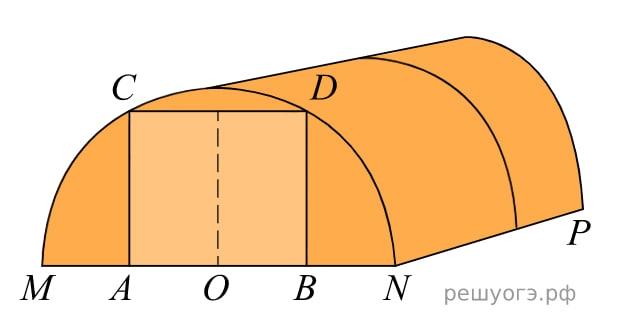
\includegraphics[align=t, width=0.5\linewidth]{\picpath/G92M6L4}
		\end{center}
		Алексей Юрьевич решил построить на дачном участке теплицу длиной \( NP=5,5 \) м. Для этого он сделал прямоугольный фундамент. Для каркаса теплицы Алексей Юрьевич заказывает металлические дуги в форме полуокружностей длиной \( 5,8 \) м каждая и плёнку для обтяжки. В передней стенке планируется вход, показанный на рисунке прямоугольником \( ACDB \).\\
		Точки \( A \) и \( B \) --- середины отрезков \( MO \) и \( ON \) соответственно.
		\item Найдите примерную ширину \( MN \) теплицы в метрах. Число π возьмите равным \( 3,14 \). Результат округлите до десятых.
		\item Найдите примерную площадь участка внутри теплицы в квадратных метрах. Ответ округлите до целых.
		\item Сколько квадратных метров плёнки нужно купить для теплицы с учётом передней и задней стенок, включая дверь? Для крепежа плёнку нужно покупать с запасом \( 10\% \). Число \( \pi \) возьмите равным \( 3,14 \). Ответ округлите до целых.
		\item Найдите примерную высоту входа в теплицу в метрах. Число \( \pi \) возьмите равным \( 3,14 \). Ответ округлите до десятых.
		\item Диагонали \( AC \) и \( BD \) параллелограмма \( ABCD \) пересекаются в точке \( O \), \( AC=14 \), \( BD=18 \), \( AB=5 \). Найдите \( DO \).
		\item Площадь ромба равна \( 54 \), а периметр равен \( 36 \). Найдите высоту ромба.
		\item Трапеция \( ABCD \) с основаниями \( AD \) и \( BC \) описана около окружности, \( AB=7 \), \( BC=5 \), \( CD=17 \). Найдите \( AD \).
		\item На окружности с центром \( O \) отмечены точки \( A \) и \( B \) так, что \( \angle AOB=18\degree \). Длина меньшей дуги \( AB \) равна \( 98 \). Найдите длину большей дуги.
		\item Отрезки \( AB \) и \( CD \) являются хордами окружности. Найдите расстояние от центра окружности до хорды \( CD \), если \( AB=12 \), \( CD=16 \), а расстояние от центра окружности до хорды \( AB \) равно \( 8 \).
		\item Радиус вписанной в квадрат окружости равен \( 26\sqrt{2} \). Найдите радиус окружности, описанной около этого квадрата.
		\item В треугольнике \( ABC \) угол \( B \) равен \( 56\degree \), угол \( C \) равен \( 64\degree \), \( BC=3\sqrt{3} \). Найдите радиус описанной около этого треугольника окружности.
		\item Окружность с центром на стороне \( AC \) треугольника \( ABC \) проходит через вершину \( C \) и касается прямой \( AB \) в точке \( B \). Найдите диаметр окружности, если \( AB=3 \), \( AC=5 \).
	\end{listofex}
\end{exam}
%END_FOLD